%!TEX root = ../report.tex
\chapter{Visual Design}

To create a visually aesthetic application we have taken into account several preparation steps upfront. In this chapter
we will go into more detail on which steps have been accomplished and how they helped us to implement our frontend parts
later on.

\section{Grid \& Measurements}\label{sec:grid-and-measurements}

It started with defining a grid and measurements guide for arranging all application components. For this we created a
grid visualization (Figure~\ref{fig:grid}).

\begin{figure}[!ht]
    \centering
    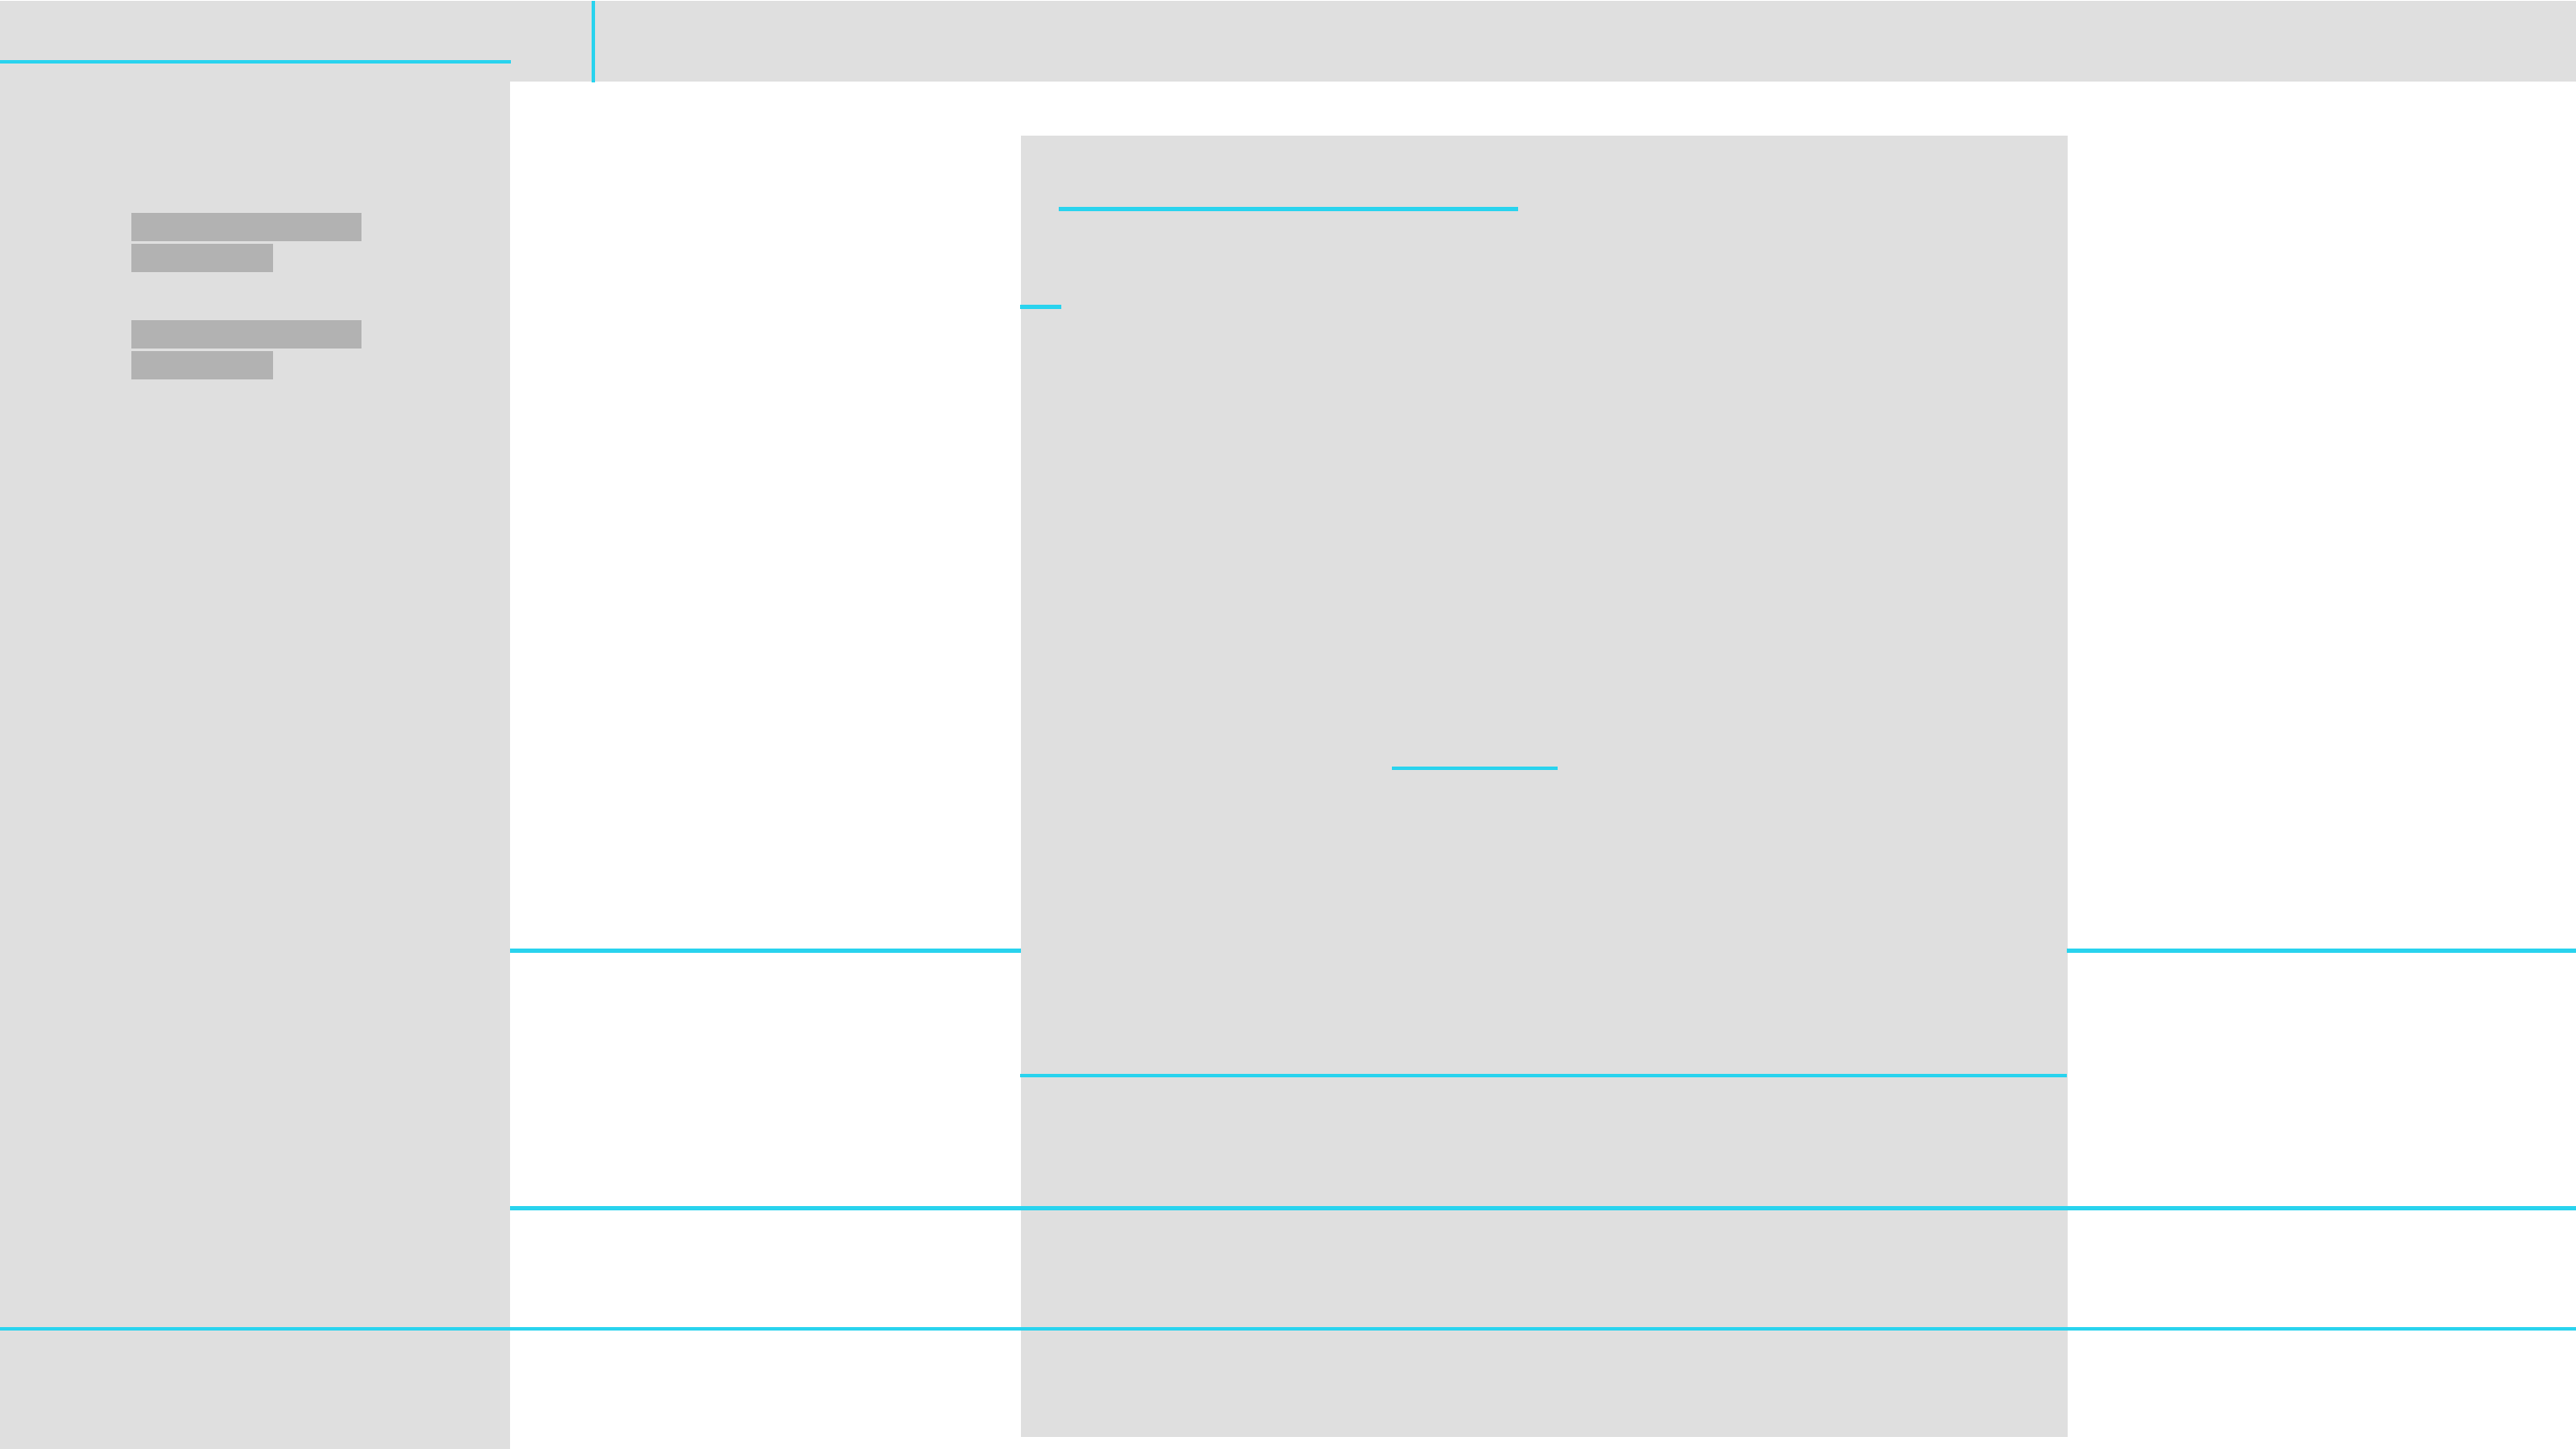
\includegraphics[width=1.0\textwidth]{./images/grid.pdf}
    \caption{Grid and Measurements visualization}
    \label{fig:grid}
\end{figure}
